% !TeX program = xelatex
\ifdefined\BookMaster\else
\documentclass[11pt,oneside]{article}
% !TeX program = xelatex
\usepackage[b5paper,left=22mm,right=22mm,top=20mm,bottom=22mm,footskip=11mm]{geometry}
\usepackage{fontspec}
\setmainfont{TeX Gyre Termes}
\setsansfont{TeX Gyre Heros}
\usepackage{amsmath,amssymb,mathtools,amsthm}
\renewcommand{\cdots}{\mathinner{\cdotp\cdotp\cdotp}}
\usepackage{graphicx,adjustbox,array,booktabs,longtable,multirow,enumitem,changepage,needspace}
\usepackage[table]{xcolor}
\usepackage{fancyhdr}
\raggedbottom
\interfootnotelinepenalty=10000
\newcommand{\BookFootnote}[2]{\begingroup\renewcommand{\thefootnote}{\fnsymbol{footnote}}\footnote[#1]{#2}\endgroup}
\newcommand{\BookFootnoteMark}[1]{\begingroup\renewcommand{\thefootnote}{\fnsymbol{footnote}}\footnotemark[#1]\endgroup}
\newcommand{\BookFootnoteText}[2]{\begingroup\renewcommand{\thefootnote}{\fnsymbol{footnote}}\footnotetext[#1]{#2}\endgroup}
\newenvironment{BookFloat}[1]{\par\addvspace{.6\baselineskip}\noindent\def\BookFloatID{#1}\begin{minipage}{\linewidth}\phantomsection\label{bookfloat:#1:start}}{\phantomsection\label{bookfloat:\BookFloatID:end}\end{minipage}\par\addvspace{.6\baselineskip}}

\usepackage[unicode,hidelinks]{hyperref}
\pagestyle{fancy}
\fancyhf{}
\newcommand{\BookFooter}{}
\fancyfoot[L]{\parbox[b]{\dimexpr\textwidth-15mm}{\footnotesize\BookFooter}}
\fancyfoot[R]{\footnotesize\thepage}
\renewcommand{\headrulewidth}{0pt}
\renewcommand{\footrulewidth}{0pt}
\setlength{\parindent}{0pt}
\setlength{\parskip}{0.2em}
\setlength{\emergencystretch}{3em}
\setlist{nosep,leftmargin=1.7em,labelsep=.65em}
\newif\ifBookNarrative
\BookNarrativetrue
\newenvironment{BookBody}{\setlength{\parindent}{0pt}}{}
\newcommand{\BookStatement}[1]{\par\addvspace{.6\baselineskip}\noindent #1\enspace\ignorespaces}
\newcommand{\BookLabel}[1]{\par\addvspace{.6\baselineskip}\needspace{3\baselineskip}\noindent\textbf{#1}\quad\ignorespaces}
\newcommand{\BookHeading}[1]{\par\addvspace{\baselineskip}\needspace{4\baselineskip}\noindent{\large\bfseries #1}\par\medskip}
\newcommand{\BookSubheading}[1]{\par\addvspace{.7\baselineskip}\needspace{3\baselineskip}\noindent{\bfseries #1}\par\smallskip}
\newcommand{\BookTextHeading}[1]{\par\addvspace{.7\baselineskip}\needspace{3\baselineskip}\noindent #1\par\smallskip}
\newcommand{\BookSectionTitle}[2]{\par\addvspace{1.2\baselineskip}\needspace{5\baselineskip}\noindent\colorbox{gray!25}{\sffamily\bfseries\small SECTION #1}\quad{\large\bfseries #2}\par\medskip}
\newcommand{\BookExerciseTitle}[1]{\par\addvspace{\baselineskip}\needspace{4\baselineskip}\noindent{\color{gray}\rule{1.5mm}{1.5mm}}\enspace{\large\bfseries Exercises #1}\par\medskip}
\newcommand{\BookBullet}[1]{\begin{list}{\textbullet}{\setlength{\leftmargin}{1.7em}\setlength{\labelwidth}{1em}\setlength{\labelsep}{.7em}\setlength{\topsep}{0pt}\setlength{\parsep}{0pt}\setlength{\itemsep}{0pt}}\item #1\end{list}}
\newcommand{\BookExercise}[2]{\begin{list}{\textbf{#1}}{\setlength{\leftmargin}{2.2em}\setlength{\labelwidth}{1.5em}\setlength{\labelsep}{.7em}\setlength{\topsep}{.15em}\setlength{\parsep}{0pt}\setlength{\itemsep}{0pt}}\item #2\end{list}}
\newcommand{\BookEnd}[1]{\unskip\nobreak\hfill\ensuremath{#1}}
\newcommand{\BookSource}[2]{\phantomsection\label{sourcepage:#1}} % Source-page anchors, retained through reflow.
\usepackage{multicol}
\usepackage{tikz}
\newcommand{\BookPartEntry}[2]{\par\noindent\makebox[17mm][l]{\bfseries Section #1}#2\par}
\newcommand{\BookPartTitle}[3]{\par\bigskip\noindent\begin{tikzpicture}\node[anchor=north west,inner sep=0pt,outer sep=0pt] (bookpart) at (0,0) {\begin{minipage}{\dimexpr\linewidth-.5pt}\hspace*{26mm}\begin{minipage}[t]{\dimexpr\linewidth-26mm}\begin{adjustbox}{max width=\linewidth}{\fontsize{20}{24}\selectfont\bfseries #2}\end{adjustbox}\par\vspace{6mm}\hrule\vspace{6mm}{\sffamily\footnotesize\setlength{\parskip}{.3em}#3}\vspace{3mm}\end{minipage}\end{minipage}};\path[shade,top color=gray!60,bottom color=white] (0,0) rectangle ([xshift=24mm]bookpart.south west);\node[anchor=north,font=\sffamily\bfseries\small] at (12mm,-2mm) {PART};\node[anchor=north,font=\sffamily\bfseries\Huge] at (12mm,-7mm) {#1};\end{tikzpicture}\par\bigskip}
\newsavebox{\BookMathBox}
\makeatletter
\newcommand{\BookInline}[1]{\leavevmode\hskip0pt\relax\begingroup\in@{\begin}{#1}\ifin@\sbox{\BookMathBox}{\(#1\)}\ifdim\wd\BookMathBox>\dimexpr\linewidth-1em\relax\resizebox{\dimexpr\linewidth-1em\relax}{!}{\usebox{\BookMathBox}}\else\(#1\)\fi\else\in@{\left}{#1}\ifin@\sbox{\BookMathBox}{\(#1\)}\ifdim\wd\BookMathBox>\dimexpr\linewidth-1em\relax\resizebox{\dimexpr\linewidth-1em\relax}{!}{\usebox{\BookMathBox}}\else\(#1\)\fi\else\(#1\)\fi\fi\endgroup\hskip0pt\relax}
\makeatother
\DeclareMathOperator{\Aut}{Aut}
\DeclareMathOperator{\End}{End}
\DeclareMathOperator{\Hom}{Hom}
\DeclareMathOperator{\GF}{GF}
\DeclareMathOperator{\irr}{irr}
\DeclareMathOperator{\lt}{lt}
\DeclareMathOperator{\lp}{lp}
\providecommand{\textcircled}[1]{\textnormal{(#1)}}

\begin{document}
\fi
\renewcommand{\BookFooter}{Section 6 Cyclic Groups}
\pdfbookmark[0]{Section 6 Cyclic Groups}{06_cyclic_groups}
\ifdefined\BookMaster\else\setcounter{page}{61}\fi
% Source PDF page 78; original printed page 61
\BookSource{78}{61}
\BookNarrativetrue

\begin{BookBody}

\BookSectionTitle{6}{Cyclic Groups}

\noindent Recall the following facts and notations from Section 5. If \BookInline{G} is a group and \BookInline{a\in G,\allowbreak } then

\begin{center}\begin{adjustbox}{max width=\linewidth}\BookInline{\displaystyle H= \{a^{n}\mid n\in \mathbb{Z}\}}\end{adjustbox}\end{center}

\noindent is a subgroup of \BookInline{G(}Theorem 5.19). This group is the\textbf{ cyclic subgroup} \BookInline{\langle a\rangle } \textbf{of} \BookInline{G} \textbf{gener}\textbf{ated by} \BookInline{a.} Also, given a group \BookInline{G} and an element \BookInline{a} in \BookInline{G,\allowbreak } if

\begin{center}\begin{adjustbox}{max width=\linewidth}\BookInline{\displaystyle G= \{a^{n}\mid n\in \mathbb{Z}\},\allowbreak }\end{adjustbox}\end{center}

\noindent then \BookInline{a} is a\textbf{ generator of} \BookInline{G} and the group \BookInline{G= \langle a\rangle } is\textbf{ cyclic.} We introduce one new bit of terminology. Let \BookInline{a} be an element of a group \BookInline{G.} If the cyclic subgroup \BookInline{\langle a\rangle } of \BookInline{G} is finite, then the\textbf{ order of} \BookInline{a} is the order \BookInline{|\langle a\rangle |} of this cyclic subgroup. Otherwise, we say that \BookInline{a} is of\textbf{ infinite order.} We will see in this section that if \BookInline{a\in G} is of finite order \BookInline{m,\allowbreak } then \BookInline{m} is the smallest positive integer such that \BookInline{a^{m}= e.}

The first goal of this section is to describe all cyclic groups and all subgroups of cyclic groups. This is not an idle exercise. We will see later that cyclic groups serve as building blocks for a significant class of abelian groups, in particular, for all finite abelian groups. Cyclic groups are fundamental to the understanding of groups.

\BookTextHeading{\textbf{Elementary Properties of Cyclic Groups}  }

\noindent We start with a demonstration that cyclic groups are abelian.

\BookLabel{6.1 Theorem} Every cyclic group is abelian.

\BookLabel{\textit{Proof}} Let \BookInline{G} be a cyclic group and let \BookInline{a} be a generator of \BookInline{G} so that

\begin{center}\begin{adjustbox}{max width=\linewidth}\BookInline{\displaystyle G= \langle a\rangle = \{a^{n}\mid n\in \mathbb{Z}\}.}\end{adjustbox}\end{center}

\noindent If \BookInline{g_{1}} and \BookInline{g_{2}} are any two elements of \BookInline{G,\allowbreak } there exist integers \BookInline{r} and \BookInline{s} such that \BookInline{g_{1}= a^{r}} and \BookInline{g_{2}= a^{s}.} Then

\begin{center}\begin{adjustbox}{max width=\linewidth}\BookInline{\displaystyle g_{1}g_{2}= a^{r}a^{s}= a^{r+ s}= a^{s+ r}= a^{s}a^{r}= g_{2}g_{1},\allowbreak }\end{adjustbox}\end{center}

\noindent so \BookInline{G} is abelian. \BookEnd{\blacklozenge}

We shall continue to use multiplicative notation for our general work on cyclic groups, even though they are abelian.

The\textit{ division algorithm} that follows is well known and seems pretty simple. In fact, this algorithm is taught in elementary school. If you divide an integer \BookInline{n} by a positive integer \BookInline{m,\allowbreak } you get an integer quotient \BookInline{q} with a remainder \BookInline{r} where \BookInline{0\leq r<m.} You might write this as \BookInline{n\div m= q} R \BookInline{r,\allowbreak } which of course means \BookInline{\begin{array} { r } { \frac { n } { m } = q + \frac { r } { m } } \end{array}}. Multiplying both sides by \BookInline{m} gives the form of the division algorithm that is a fundamental tool for the study of cyclic groups.

\end{BookBody}

% Source PDF page 79; original printed page 62
\BookSource{79}{62}
\BookNarrativetrue

\begin{BookBody}

\BookExercise{6.}{\textbf{6.2 Division Algorithm for} \BookInline{\mathbb{Z}} If \BookInline{m} is a positive integer and \BookInline{n} is any integer, then there exist unique integers \BookInline{q} and \BookInline{r} such that}

\begin{center}\begin{adjustbox}{max width=\linewidth}\BookInline{\displaystyle n= mq+ r\;\text{and}\;0\leq r<m.}\end{adjustbox}\end{center}

\BookLabel{\textit{Proof}} We give an intuitive diagrammatic explanation, using Fig. 6.3. On the number line, mark off the multiples of \BookInline{m} and the position of \BookInline{n.} Now \BookInline{n} falls either on a multiple \BookInline{qm} of \BookInline{m} and \BookInline{r} can be taken as 0, or \BookInline{n} falls between two multiples of \BookInline{m.} If the latter is the case, let \BookInline{qm} be the first multiple of \BookInline{m} to the left of \BookInline{n.} Then \BookInline{r} is as shown in Fig. 6.3. Note that \BookInline{0\leq r<m.} Uniqueness of \BookInline{q} and \BookInline{r} follows since if \BookInline{n} is not a multiple of \BookInline{m} so that we can take \BookInline{r= 0,\allowbreak } then there is a unique multiple \BookInline{qm} of \BookInline{m} to the left of \BookInline{n} and at distance less than \BookInline{m} from \BookInline{n,\allowbreak } as illustrated in Fig\BookInline{.6.3.}\BookEnd{\blacklozenge}

\begin{BookFloat}{06_cyclic_groups-p79-3}
\begin{center}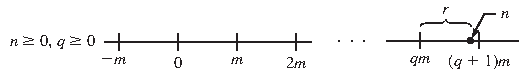
\includegraphics[width=0.717\linewidth,height=.8\textheight,keepaspectratio]{assets/p079_07.pdf}\end{center}
\end{BookFloat}

\begin{BookFloat}{06_cyclic_groups-p79-4}
\begin{center}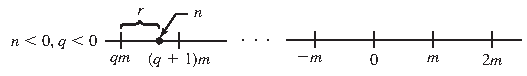
\includegraphics[width=0.723\linewidth,height=.8\textheight,keepaspectratio]{assets/p079_08.pdf}\end{center}
\begin{center}\small\textbf{6.3 Figure}\end{center}
\end{BookFloat}

In the notation of the division algorithm, we regard \BookInline{q} as the\textbf{ quotient} and \BookInline{r} as the nonnegative\textbf{ remainder} when \BookInline{n} is divided by \BookInline{m.}

\BookLabel{6.4 Example} Find the quotient \BookInline{q} and remainder \BookInline{r} when 38 is divided by 7 according to the division algorithm.

\BookLabel{\textit{Solution}} The positive multiples of 7 are \BookInline{7,\allowbreak 14,\allowbreak 21,\allowbreak 28,\allowbreak 35,\allowbreak 42,\allowbreak \cdots.} Choosing the multiple to leave a nonnegative remainder less than 7, we write

\begin{center}\begin{adjustbox}{max width=\linewidth}\BookInline{\displaystyle 38= 35+ 3= 7(5)+ 3}\end{adjustbox}\end{center}

\noindent so the quotient is \BookInline{q= 5} and the remainder is \BookInline{r= 3.} \BookEnd{\blacktriangle}

\BookLabel{6.5 Example} Find the quotient \BookInline{q} and remainder \BookInline{r} when \BookInline{- 38} is divided by 7 according to the division algorithm.

\BookLabel{\textit{Solution}} The negative multiples of 7 are \BookInline{- 7,\allowbreak - 14,\allowbreak - 21,\allowbreak - 28,\allowbreak - 35,\allowbreak - 42,\allowbreak \cdots.} Choosing the multiple to leave a nonnegative remainder less than 7, we write

\begin{center}\begin{adjustbox}{max width=\linewidth}\BookInline{\displaystyle - 38= - 42+ 4= 7(- 6)+ 4}\end{adjustbox}\end{center}

\noindent so the quotient is \BookInline{q= - 6} and the remainder is \BookInline{r= 4.} \BookEnd{\blacktriangle}

We will use the division algorithm to show that a subgroup \BookInline{H} of a cyclic group \BookInline{G} is also cyclic. Think for a moment what we will have to do to prove this. We will have to use the\textit{ definition} of a cyclic group since we have proved little about cyclic groups yet. That is, we will have to use the fact that \BookInline{G} has a generating element \BookInline{a.} We must then exhibit, in terms of this generator \BookInline{a,\allowbreak } some generator \BookInline{c= a^{m}} for \BookInline{H} in order to show that \BookInline{H} is cyclic. There is really only one natural choice for the power \BookInline{m} of \BookInline{a} to try. Can you guess what it is before you read the proof of the theorem?

\end{BookBody}

% Source PDF page 80; original printed page 63
\BookSource{80}{63}
\BookNarrativetrue

\begin{BookBody}

\BookLabel{6.6 Theorem} A subgroup of a cyclic group is cyclic.

\BookLabel{\textit{Proof}} Let \BookInline{G} be a cyclic group generated by \BookInline{a} and let \BookInline{H} be a subgroup of \BookInline{G.} If \BookInline{H= \{e\},\allowbreak } then \BookInline{H= \langle e\rangle } is cyclic. If \BookInline{H\neq \{e\},\allowbreak } then \BookInline{a^{n}\in H} for some \BookInline{n\in \mathbb{Z}^{+ }.} Let \BookInline{m} be the smallest integer in \BookInline{\mathbb{Z}^{+ }} such that \BookInline{a^{m}\in H.}

We claim that \BookInline{c= a^{m}} generates \BookInline{H;} that is,

\begin{center}\begin{adjustbox}{max width=\linewidth}\BookInline{\displaystyle H= \langle a^{m}\rangle = \langle c\rangle .}\end{adjustbox}\end{center}

\noindent We must show that every \BookInline{b\in H} is a power of \BookInline{c.} Since \BookInline{b\in H} and \BookInline{H\leq G,\allowbreak } we have \BookInline{b= a^{n}} for some \BookInline{n.} Find \BookInline{q} and \BookInline{r} such that

\begin{center}\begin{adjustbox}{max width=\linewidth}\BookInline{\displaystyle n= mq+ r\;\text{for}\;0\leq r<m}\end{adjustbox}\end{center}

\noindent in accord with the division algorithm. Then

\begin{center}\begin{adjustbox}{max width=\linewidth}\BookInline{\displaystyle a^{n}= a^{mq+ r}= (a^{m})^{q}a^{r},\allowbreak }\end{adjustbox}\end{center}

\noindent so

\begin{center}\begin{adjustbox}{max width=\linewidth}\BookInline{\displaystyle a^{r}= (a^{m})^{- q}a^{n}.}\end{adjustbox}\end{center}

\noindent Now since \BookInline{a^{n}\in H,\allowbreak a^{m}\in H,\allowbreak } and \BookInline{H} is a group, both \BookInline{(a^{m})^{- q}} and \BookInline{a^{n}} are in \BookInline{H.} Thus

\begin{center}\begin{adjustbox}{max width=\linewidth}\BookInline{\displaystyle (a^{m})^{- q}a^{n}\in H;\;\text{that is}\;,\allowbreak a^{r}\in H.}\end{adjustbox}\end{center}

\noindent Since \BookInline{m} was the smallest positive integer such that \BookInline{a^{m}\in H} and \BookInline{0\leq r<m,\allowbreak } we must have \BookInline{r= 0.} Thus \BookInline{n= mq} and

\begin{center}\begin{adjustbox}{max width=\linewidth}\BookInline{\displaystyle b= a^{n}= (a^{m})^{q}= c^{q},\allowbreak }\end{adjustbox}\end{center}

\noindent so \BookInline{b} is a power of \BookInline{c.} \BookEnd{\blacklozenge}

As noted in Examples 5.24 and \BookInline{5.25,\allowbreak \mathbb{Z}} under addition is cyclic and for a positive integer \BookInline{n,\allowbreak } the set \BookInline{n\mathbb{Z}} of all multiples of \BookInline{n} is a subgroup of \BookInline{\mathbb{Z}} under addition, the cyclic subgroup generated by \BookInline{n.} Theorem 6.6 shows that these cyclic subgroups are the only subgroups of \BookInline{\mathbb{Z}} under addition. We state this as a corollary.

\BookLabel{6.7 Corollary} The subgroups of \BookInline{\mathbb{Z}} under addition are precisely the groups \BookInline{n\mathbb{Z}} under addition for \BookInline{n\in \mathbb{Z}.} \BookEnd{\blacklozenge}

This corollary gives us an elegant way to define the\textit{ greatest common divisor} of two positive integers \BookInline{r} and \BookInline{s.} Exercise 54 shows that \BookInline{H= \{nr+ ms\mid n,\allowbreak m\in \mathbb{Z}\}} is a subgroup of the group \BookInline{\mathbb{Z}} under addition. Thus \BookInline{H} must be cyclic and have a generator \BookInline{d,\allowbreak } which we may choose to be positive.

\BookLabel{6.8 Definition} Let \BookInline{r} be a positive integer and \BookInline{s} be a non-negative integer. The positive generator \BookInline{d} of the cyclic group

\begin{center}\begin{adjustbox}{max width=\linewidth}\BookInline{\displaystyle H= \{nr+ ms\mid n,\allowbreak m\in \mathbb{Z}\}}\end{adjustbox}\end{center}

\noindent under addition is the\textbf{ greatest common divisor} (abbreviated gcd) of \BookInline{r} and \BookInline{s.} We write \BookInline{d= } gcd\BookInline{(r,\allowbreak s).}\BookEnd{\blacksquare}

Note that \BookInline{d\mathbb{Z}= H,\allowbreak r= 1r+ 0s\in H,\allowbreak } and \BookInline{s= 0r+ 1s\in H.} This implies that \BookInline{r,\allowbreak s\in } \BookInline{d\mathbb{Z},\allowbreak } which says that \BookInline{d} is a divisor of both \BookInline{r} and \BookInline{s.} Since \BookInline{d\in H,\allowbreak } we can write

\begin{center}\begin{adjustbox}{max width=\linewidth}\BookInline{\displaystyle d= nr+ ms}\end{adjustbox}\end{center}

\noindent for some integers \BookInline{n} and \BookInline{m.} We see that every integer dividing both \BookInline{r} and \BookInline{s} divides the right-hand side of the equation, and hence must be a divisor of \BookInline{d} also. Thus \BookInline{d} must 
% Source PDF page 81; original printed page 64
\BookSource{81}{64}
be the largest number dividing both \BookInline{r} and \BookInline{s;} this accounts for the name given to \BookInline{d} in Definition 6.8.

\end{BookBody}

\BookNarrativetrue

\begin{BookBody}

The fact that the greatest common divisor \BookInline{d} of \BookInline{r} and \BookInline{s} can be written in the form \BookInline{d= nr+ ms} for some integers \BookInline{n} and \BookInline{m} is called Be´zout’s identity. Be´zout’s identity is very useful in number theory, as we will see in studying cyclic groups.

\BookLabel{6.9 Example} Find the gcd of 42 and 72.

\BookLabel{\textit{Solution}} The positive divisors of 42 are 1, 2, 3, 6, 7, 14, 21, and 42. The positive divisors of 72 are 1, 2, 3, 4, 6, 8, 9, 12, 18, 24, 36, and 72. The greatest common divisor is 6. Note that \BookInline{6= (3)(72)+ (- 5)(42).} There is an algorithm for expressing the greatest common divisor \BookInline{d} of \BookInline{r} and \BookInline{s} in the form \BookInline{d= nr+ ms,\allowbreak } but we will not need to make use of it here. The interested reader can find the algorithm by searching the Internet for the Euclidean algorithm and Be´zout’s identity\BookInline{.}\BookEnd{\blacktriangle}

Two positive integers are\textbf{ relatively prime} if their gcd is 1. For example, 12 and 25 are relatively prime. Note that they have no prime factors in common. In our discussion of subgroups of cyclic groups, we will need to know the following:

If \BookInline{r} and \BookInline{s} are relatively prime and if \BookInline{r} divides \BookInline{sm,\allowbreak } then \BookInline{r} must divide \BookInline{m.(1)}

\noindent Let’s prove this. If \BookInline{r} and \BookInline{s} are relatively prime, then we may write

\begin{center}\begin{adjustbox}{max width=\linewidth}\BookInline{\displaystyle 1= ar+ bs\;\text{for some}\;a,\allowbreak b\in \mathbb{Z}.}\end{adjustbox}\end{center}

\noindent Multiplying by \BookInline{m,\allowbreak } we obtain

\begin{center}\begin{adjustbox}{max width=\linewidth}\BookInline{\displaystyle m= arm+ bsm.}\end{adjustbox}\end{center}

\noindent Now \BookInline{r} divides both \BookInline{arm} and \BookInline{bsm} since \BookInline{r} divides \BookInline{sm.} Thus \BookInline{r} is a divisor of the right-hand side of this equation, so \BookInline{r} must divide \BookInline{m.}

\BookTextHeading{\textbf{The Structure of Cyclic Groups}  }

\noindent We can now describe all cyclic groups, up to an isomorphism.

\BookLabel{6.10 Theorem} Let \BookInline{G} be a cyclic group with generator \BookInline{a.} If the order of \BookInline{G} is infinite, then \BookInline{G} is isomorphic to \BookInline{\langle \mathbb{Z},\allowbreak + \rangle.} If \BookInline{G} has finite order \BookInline{n,\allowbreak } then \BookInline{G} is isomorphic to \BookInline{\langle \mathbb{Z}_{n},\allowbreak + _{n}\rangle.}

\BookLabel{\textit{Proof}} \textbf{Case I} \textit{For all positive integers} \BookInline{m,\allowbreak } \BookInline{a ^ { m } \neq e.} In this case we claim that no two distinct exponents \BookInline{h} and \BookInline{k} can give equal elements \BookInline{a^{h}} and \BookInline{a^{k}} of \BookInline{G.} Suppose that \BookInline{a^{h}= a^{k}} and say \BookInline{h>k.} Then

\begin{center}\begin{adjustbox}{max width=\linewidth}\BookInline{\displaystyle a^{h}a^{- k}= a^{h- k}= e,\allowbreak }\end{adjustbox}\end{center}

contrary to our Case I assumption. Hence every element of \BookInline{G} can be expressed as \BookInline{a^{m}} for a unique \BookInline{m\in \mathbb{Z}.} The map \BookInline{\phi:G\to \mathbb{Z}} given by \BookInline{\phi (a^{i})= i} is thus well defined, one-to-one, and onto \BookInline{\mathbb{Z}.} Also,

\begin{center}\begin{adjustbox}{max width=\linewidth}\BookInline{\displaystyle \phi (a^{i}a^{j})= \phi (a^{i+ j})= i+ j= \phi (a^{i})+ \phi (a^{j}),\allowbreak }\end{adjustbox}\end{center}

so the homomorphism property is satisfied and \BookInline{\phi } is an isomorphism.

\end{BookBody}

% Source PDF page 82; original printed page 65
\BookSource{82}{65}
\BookNarrativetrue

\begin{BookBody}

\textbf{Case II} \BookInline{a^{m}= e} \textit{for some positive integer} \BookInline{m.} Let \BookInline{n} be the smallest positive integer such that \BookInline{a^{n}= e.} If \BookInline{s\in \mathbb{Z}} and \BookInline{s= nq+ r} for \BookInline{0\leq r<n,\allowbreak } then \BookInline{a^{s}= a^{nq+ r}= (a^{n})^{q}a^{r}= e^{q}a^{r}= a^{r}.} As in Case 1, if \BookInline{0\leq k<h<n} and \BookInline{a^{h}= a^{k},\allowbreak } then \BookInline{a^{h- k}= e} and \BookInline{0<h- k<n,\allowbreak } contradicting our choice of \BookInline{n.} Thus the elements

\begin{center}\begin{adjustbox}{max width=\linewidth}\BookInline{\displaystyle a^{0}= e,\allowbreak a,\allowbreak a^{2},\allowbreak a^{3},\allowbreak \cdots ,\allowbreak a^{n- 1}}\end{adjustbox}\end{center}

are all distinct and comprise all elements of \BookInline{G.} The map \BookInline{\psi:G\to \mathbb{Z}_{n}} given by \BookInline{\psi (a^{i})= i} for \BookInline{i= 0,\allowbreak 1,\allowbreak 2,\allowbreak \cdots,\allowbreak n- 1} is thus well defined, one-to-one, and onto \BookInline{\mathbb{Z}_{n}.} Because \BookInline{a^{n}= e,\allowbreak } we see that \BookInline{a^{i}a^{j}= a^{k}} where \BookInline{k= i+ _{n}j.} Thus

\begin{center}\begin{adjustbox}{max width=\linewidth}\BookInline{\displaystyle \psi (a^{i}a^{j})= i+ _{n}j= \psi (a^{i})+ _{n}\psi (a^{j}),\allowbreak }\end{adjustbox}\end{center}

so the homomorphism property is satisfied and \BookInline{\psi } is an isomorphism. \BookEnd{\blacklozenge}

\begin{BookFloat}{06_cyclic_groups-p82-6}
\begin{center}
\begin{minipage}[t]{0.4820\linewidth}\vspace{0pt}\begin{center}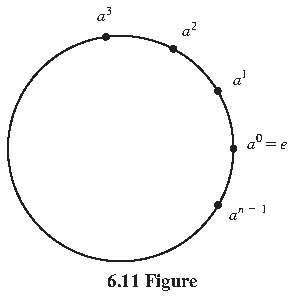
\includegraphics[width=\linewidth,height=.8\textheight,keepaspectratio]{assets/p082_06.pdf}\end{center}\end{minipage}\hfill\begin{minipage}[t]{0.4565\linewidth}\vspace{0pt}\begin{center}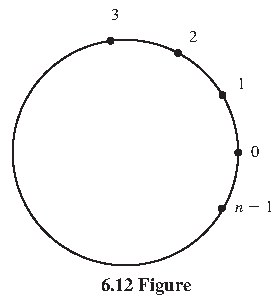
\includegraphics[width=\linewidth,height=.8\textheight,keepaspectratio]{assets/p082_07.pdf}\end{center}\end{minipage}
\end{center}
\end{BookFloat}

\BookLabel{6.13 Example} Motivated by our work with \BookInline{U_{n},\allowbreak } it is nice to visualize the elements \BookInline{e= a^{0},\allowbreak a^{1},\allowbreak a^{2},\allowbreak \cdots,\allowbreak } \BookInline{a^{n- 1}} of a cyclic group of order \BookInline{n} as being distributed evenly on a circle (see Fig. 6.11). The element \BookInline{a^{h}} is located \BookInline{h} of these equal units counterclockwise along the circle, measured from the right where \BookInline{e= a^{0}} is located. To multiply \BookInline{a^{h}} and \BookInline{a^{k}} diagrammatically, we start from \BookInline{a^{h}} and go \BookInline{k} additional units around counterclockwise. To see arithmetically where we end up, find \BookInline{q} and \BookInline{r} such that

\begin{center}\begin{adjustbox}{max width=\linewidth}\BookInline{\displaystyle h+ k= nq+ r\;\text{for}\;0\leq r<n.}\end{adjustbox}\end{center}

\noindent The \BookInline{nq} takes us all the way around the circle \BookInline{q} times, and we then wind up at \BookInline{a^{r}.}\BookEnd{\blacktriangle}

Figure 6.12 is essentially the same as Fig. 6.11 but with the points labeled with the exponents on the generator. The operation on these exponents is\textit{ addition modulo} \BookInline{n.}

This is simply the isomorphism between \BookInline{\langle a\rangle } and \BookInline{\mathbb{Z}_{n}.} Of course this is the same isomorphism we saw when we defined \BookInline{\mathbb{Z}_{n}} from \BookInline{U_{n},\allowbreak } but using \BookInline{a} instead of \BookInline{\zeta.}

As promised at the beginning of this section, we can see now that the order of an element \BookInline{a} in a group \BookInline{G} is simply the smallest positive number \BookInline{n} such that \BookInline{a^{n}= e.}

\BookLabel{6.14 Example} Let us find the order of the \BookInline{k-}cycle\BookInline{,\allowbreak \sigma = (a_{1},\allowbreak a_{2},\allowbreak a_{3},\allowbreak...,\allowbreak a_{k}),\allowbreak } in the symmetric group. The order of \BookInline{\sigma } is the smallest postive power of \BookInline{\sigma } that is \BookInline{\iota.} Note that applying \BookInline{\sigma } just maps each number to the next one in the cyclic order. So after \BookInline{k} applications of \BookInline{\sigma,\allowbreak } each number maps back to itself, but not before \BookInline{k} applications of \BookInline{\sigma.} Therefore, the order of a \BookInline{k-}cycle is \BookInline{k.}\BookEnd{\blacktriangle}

\end{BookBody}

% Source PDF page 83; original printed page 66
\BookSource{83}{66}
\BookNarrativetrue

\begin{BookBody}

\BookTextHeading{\textbf{Subgroups of Finite Cyclic Groups}  }

\noindent We have completed our description of cyclic groups and turn to their subgroups. Corollary 6.7 gives us complete information about subgroups of infinite cyclic groups. Let us give the basic theorem regarding generators of subgroups for the finite cyclic groups.

\BookLabel{6.15 Theorem} Let \BookInline{G} be a cyclic group with \BookInline{n} elements and generated by \BookInline{a.} Let \BookInline{b\in G} and let \BookInline{b= a^{s}.} Then \BookInline{b} generates a cyclic subgroup \BookInline{H} of \BookInline{G} containing \BookInline{n/d} elements, where \BookInline{d} is the greatest common divisor of \BookInline{n} and \BookInline{s.} Also\BookInline{,\allowbreak \langle a^{s}\rangle = \langle a^{t}\rangle } if and only if gcd\BookInline{(s,\allowbreak n)= } gcd\BookInline{(t,\allowbreak n).}

\BookLabel{\textit{Proof}} That \BookInline{b} generates a cyclic subgroup \BookInline{H} of \BookInline{G} is known from Theorem 5.19. We need show only that \BookInline{H} has \BookInline{n/d} elements. Following the argument of Case II of Theorem 6.10, we see that \BookInline{H} has as many elements as the smallest positive power \BookInline{m} of \BookInline{b} that gives the identity. Now \BookInline{b= a^{s},\allowbreak } and \BookInline{b^{m}= e} if and only if \BookInline{(a^{s})^{m}= e,\allowbreak } or if and only if \BookInline{n} divides \BookInline{ms.} What is the smallest positive integer \BookInline{m} such that \BookInline{n} divides \BookInline{ms}? Let \BookInline{d} be the gcd of \BookInline{n} and \BookInline{s.} Then there exist integers \BookInline{u} and \BookInline{v} such that

\begin{center}\begin{adjustbox}{max width=\linewidth}\BookInline{\displaystyle d= un+ vs.}\end{adjustbox}\end{center}

\noindent Since \BookInline{d} divides both \BookInline{n} and \BookInline{s,\allowbreak } we may write

\begin{center}\begin{adjustbox}{max width=\linewidth}\BookInline{\displaystyle 1= u(n/d)+ v(s/d)}\end{adjustbox}\end{center}

\noindent where both \BookInline{n/d} and \BookInline{s/d} are integers. This last equation shows that \BookInline{n/d} and \BookInline{s/d} are relatively prime, for any integer dividing both of them must also divide 1. We wish to find the smallest positive \BookInline{m} such that

\begin{center}\begin{adjustbox}{max width=\linewidth}\BookInline{\displaystyle { \frac { m s } { n } } = { \frac { m ( s / d ) } { ( n / d ) } } { \mathrm { ~ i s ~ a n ~ i n t e g e r } } .}\end{adjustbox}\end{center}

\noindent From the division property (1) following Example 6.9, we conclude that \BookInline{n/d} must divide \BookInline{m,\allowbreak } so the smallest such \BookInline{m} is \BookInline{n/d.} Thus the order of \BookInline{H} is \BookInline{n/d.}

Taking for the moment \BookInline{\mathbb{Z}_{n}} as a model for a cyclic group of order \BookInline{n,\allowbreak } we see that if \BookInline{d} is a divisor of \BookInline{n,\allowbreak } then the cyclic subgroup \BookInline{\langle d\rangle } of \BookInline{\mathbb{Z}_{n}} has \BookInline{n/d} elements, and contains all the positive integers \BookInline{m} less than \BookInline{n} such that gcd\BookInline{(m,\allowbreak n)= d.} Thus there is only one subgroup of \BookInline{\mathbb{Z}_{n}} of order \BookInline{n/d.} Taken with the preceding paragraph, this shows at once that if \BookInline{a} is a generator of the cyclic group \BookInline{G,\allowbreak } then \BookInline{\langle a^{s}\rangle = \langle a^{t}\rangle } if and only if gcd\BookInline{(s,\allowbreak n)= } gcd\BookInline{(t,\allowbreak n).}\BookEnd{\blacklozenge}

\BookLabel{6.16 Example} For an example using additive notation, consider \BookInline{\mathbb{Z}_{12},\allowbreak } with the generator \BookInline{a= 1.} Since the greatest common divisor of 3 and 12 is \BookInline{3,\allowbreak 3= 3\cdot 1} generates a subgroup of \BookInline{\textstyle { \frac { 1 2 } { 3 } } = 4} elements, namely

\begin{center}\begin{adjustbox}{max width=\linewidth}\BookInline{\displaystyle \langle 3\rangle = \{0,\allowbreak 3,\allowbreak 6,\allowbreak 9\}.}\end{adjustbox}\end{center}

\noindent Since the gcd of 8 and 12 is 4, 8 generates a subgroup of \BookInline{\textstyle { \frac { 1 2 } { 4 } } = 3} elements, namely,

\begin{center}\begin{adjustbox}{max width=\linewidth}\BookInline{\displaystyle \langle 8\rangle = \{0,\allowbreak 4,\allowbreak 8\}.}\end{adjustbox}\end{center}

\noindent Since the gcd of 12 and 5 is 1, 5 generates a subgroup of \BookInline{\textstyle { \frac { 1 2 } { 1 } } = 1 2} elements; that is, 5 is a generator of the whole group \BookInline{\mathbb{Z}_{12}.}\BookEnd{\blacktriangle}

The following corollary follows immediately from Theorem 6.15.

\BookLabel{6.17 Corollary} If \BookInline{a} is a generator of a finite cyclic group \BookInline{G} of order \BookInline{n,\allowbreak } then the other generators of \BookInline{G} are the elements of the form \BookInline{a^{r},\allowbreak } where \BookInline{r} is relatively prime to \BookInline{n.}

\end{BookBody}

% Source PDF page 84; original printed page 67
\BookSource{84}{67}
\BookNarrativetrue

\begin{BookBody}

\BookLabel{6.18 Example} Let us find all subgroups of \BookInline{\mathbb{Z}_{18}} and give their subgroup diagram. All subgroups are cyclic. By Corollary 6.17, the elements 1, 5, 7, 11, 13, and 17 are all generators of \BookInline{\mathbb{Z}_{18}.} Starting with 2,

\begin{center}\begin{adjustbox}{max width=\linewidth}\BookInline{\displaystyle \langle 2\rangle = \{0,\allowbreak 2,\allowbreak 4,\allowbreak 6,\allowbreak 8,\allowbreak 10,\allowbreak 12,\allowbreak 14,\allowbreak 16\}.}\end{adjustbox}\end{center}

\noindent is of order 9 and has as generators elements of the form \BookInline{h2,\allowbreak } where \BookInline{h} is relatively prime to 9, namely\BookInline{,\allowbreak h= 1,\allowbreak 2,\allowbreak 4,\allowbreak 5,\allowbreak 7,\allowbreak } and 8, so \BookInline{h2= 2,\allowbreak 4,\allowbreak 8,\allowbreak 10,\allowbreak 14,\allowbreak } and 16. The element 6 of \BookInline{\langle 2\rangle } generates \BookInline{\{0,\allowbreak 6,\allowbreak 12\},\allowbreak } and 12 also is a generator of this subgroup.

We have thus far found all subgroups generated by 0, 1, 2, 4, 5, 6, 7, 8, 10, 11, 12, 13, 14, 16, and 17. This leaves just 3, 9, and 15 to consider.

\begin{center}\begin{adjustbox}{max width=\linewidth}\BookInline{\displaystyle \langle 3\rangle = \{0,\allowbreak 3,\allowbreak 6,\allowbreak 9,\allowbreak 12,\allowbreak 15\},\allowbreak }\end{adjustbox}\end{center}

\noindent and 15 also generates this group of order 6, since \BookInline{15= 5\cdot 3,\allowbreak } and the gcd of 5 and 6 is 1. Finally,

\begin{center}\begin{adjustbox}{max width=\linewidth}\BookInline{\displaystyle \langle 9\rangle = \{0,\allowbreak 9\}.}\end{adjustbox}\end{center}

\noindent The subgroup diagram for these subgroups of \BookInline{\mathbb{Z}_{18}} is given in Fig. 6.19.

\begin{BookFloat}{06_cyclic_groups-p84-8}
\begin{center}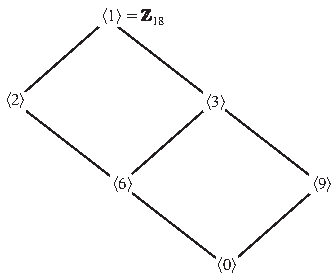
\includegraphics[width=0.459\linewidth,height=.8\textheight,keepaspectratio]{assets/p084_10.pdf}\end{center}
\begin{center}\small\textbf{6.19 Figure}\end{center}
\end{BookFloat}

Subgroup diagram for \BookInline{\mathbb{Z}_{18}.}

This example is straightforward; we are afraid we wrote it out in such detail that it may look complicated. The exercises give some practice along these lines\BookInline{.}\BookEnd{\blacktriangle}

\BookLabel{6.20 Corollary} Let \BookInline{G} be a finite cyclic group and \BookInline{H\leq G.} Then \BookInline{|H|} divides \BookInline{|G|.} That is\BookInline{,\allowbreak |G|} is a multiple of \BookInline{|H|.}

\BookLabel{\textit{Proof}} Let \BookInline{g} be a generator for \BookInline{G} and let \BookInline{n= |G|.} By Theorem \BookInline{6.6,\allowbreak H} is cyclic, so there is an element in \BookInline{h\in H} such that \BookInline{h} generates \BookInline{H.} Since \BookInline{h\in H\leq G,\allowbreak h= g^{s}} for some \BookInline{s.} Theorem 6.15 states that

\begin{center}\begin{adjustbox}{max width=\linewidth}\BookInline{\displaystyle | H | = { \frac { n } { \operatorname* { g c d } ( n ,\allowbreak  s ) } }}\end{adjustbox}\end{center}

\noindent which is a divisor of \BookInline{n.} \BookEnd{\blacklozenge}

\BookLabel{6.21 Example} We find all orders of the subgroups of \BookInline{\mathbb{Z}_{28}.} Factoring gives \BookInline{28= 2^{2}\cdot 7,\allowbreak } so the possible orders of subgroups of the cyclic group \BookInline{\mathbb{Z}_{28}} are 1, 2, 4, 7, 14, and 28. We note that \BookInline{|\langle 0\rangle |= 1,\allowbreak |\langle 14\rangle |= 2,\allowbreak |\langle 7\rangle |= 4,\allowbreak |\langle 4\rangle |= 7,\allowbreak |\langle 2\rangle |= 14,\allowbreak |\langle 1\rangle |= |\mathbb{Z}_{28}|= 28.} So there are subgroups of order 1, 2, 4, 7, 14, and \BookInline{28.}\BookEnd{\blacktriangle}

Actually, Corollary 6.20 can be strengthened considerably. The assumption that \BookInline{G} is cyclic is completely unnecessary. As we will see in Section 10, Lagrange’s Theorem states that for any finite group, the order of a subgroup divides the order of the group.

\end{BookBody}

% Source PDF page 85; original printed page 68
\BookSource{85}{68}
\BookNarrativefalse

\begin{BookBody}

\BookExerciseTitle{6}

\BookTextHeading{\textbf{Computations}}

\noindent In Exercises 1 through 4, find the quotient and remainder, according to the division algorithm, when \BookInline{n} is divided by \BookInline{m.}

\BookExercise{1.}{\BookInline{n= 42,\allowbreak m= 9}}

\BookExercise{2.}{\BookInline{n= - 42,\allowbreak m= 9}}

\BookExercise{3.}{\BookInline{n= - 37,\allowbreak m= 8}}

\BookExercise{4.}{\BookInline{n= 37,\allowbreak m= 8}}

\noindent In Exercises 5 through 7, find the greatest common divisor of the two integers.

\BookExercise{5.}{32 and 24}

\BookExercise{6.}{48 and 88}

\BookExercise{7.}{360 and 420}

\noindent In Exercises 8 through 11, find the number of generators of a cyclic group having the given order.

\BookExercise{8.}{5}

\BookExercise{9.}{8}

\BookExercise{10.}{24}

\BookExercise{11.}{84}

\noindent An isomorphism of a group with itself is an\textbf{ automorphism of the group.} In Exercises 12 through 16, find the number of automorphisms of the given group. [\textit{Hint:} You may use Exercise 53. What must be the image of a generator under an automorphism?]

\BookExercise{12.}{\BookInline{\mathbb{Z}_{2}}}

\BookExercise{13.}{\BookInline{\mathbb{Z}_{6}}}

\BookExercise{14.}{\BookInline{\mathbb{Z}_{8}}}

\BookExercise{15.}{\BookInline{\mathbb{Z}}}

\BookExercise{16.}{\BookInline{\mathbb{Z}_{84}}}

\noindent In Exercises 17 through 23, find the number of elements in the indicated cyclic group.

\BookExercise{17.}{The cyclic subgroup of \BookInline{\mathbb{Z}_{30}} generated by 25}

\BookExercise{18.}{The cyclic subgroup of \BookInline{\mathbb{Z}_{42}} generated by 30}

\BookExercise{19.}{The cyclic subgroup \BookInline{\langle i\rangle } of the group \BookInline{\mathbb{C}^{\ast }} of nonzero complex numbers under multiplication}

\BookExercise{20.}{The cyclic subgroup of the group \BookInline{\mathbb{C}^{\ast }} of Exercise 19 generated by \BookInline{(1+ i)/\sqrt{2}}}

\BookExercise{21.}{The cyclic subgroup of the group \BookInline{\mathbb{C}^{\ast }} of Exercise 19 generated by \BookInline{1+ i}}

\BookExercise{22.}{The cyclic subgroup \BookInline{\langle \rho ^{10}\rangle } of \BookInline{D_{24}}}

\BookExercise{23.}{The cyclic subgoup \BookInline{\langle \rho ^{35}\rangle } of \BookInline{D_{375}}}

\BookExercise{24.}{Consider the group \BookInline{S_{10}} \textbf{a.} What is the order of the cycle (2, 4, 6, 7)? \textbf{b.} What is the order of (1, 4)(2, 3, 5)? Of (1, 3)(2, 4, 6, 7, 8)? \textbf{c.} What is the order of (1, 5, 9)(2, 6, 7)? Of (1, 3)(2, 5, 6, 8)? \textbf{d.} What is the order of (1, 2)(3, 4, 5, 6, 7, 8)? Of (1, 2, 3)(4, 5, 6, 7, 8, 9)?}

\BookExercise{e.}{State a theorem suggested by parts (c) and (d). [Hint: The important words you are looking for are\textit{ least} \textit{common multiple}.]}

\noindent In Exercises 25 through 30, find the maximum possibe order for an element of \BookInline{S_{n}} for a given value of \BookInline{n.}

\BookExercise{25.}{\BookInline{n= 5}}

\BookExercise{26.}{\BookInline{n= 6}}

\BookExercise{27.}{\BookInline{n= 7}}

\BookExercise{28.}{\BookInline{n= 8}}

\BookExercise{29.}{\BookInline{n= 10}}

\BookExercise{30.}{\BookInline{n= 15}}

\noindent In Exercises 31 through 33, find all subgroups of the given group, and draw the subgroup diagram for the subgroups.

\BookExercise{31.}{\BookInline{\mathbb{Z}_{12}}}

\BookExercise{32.}{\BookInline{\mathbb{Z}_{36}}}

\BookExercise{33.}{\BookInline{\mathbb{Z}_{8}}}

\noindent In Exercises 34 through 38, find all orders of subgroups of the given group.

\BookExercise{34.}{\BookInline{\mathbb{Z}_{6}}}

\BookExercise{35.}{\BookInline{\mathbb{Z}_{8}}}

\BookExercise{36.}{\BookInline{\mathbb{Z}_{12}}}

\BookExercise{37.}{\BookInline{\mathbb{Z}_{20}}}

\BookExercise{38.}{\BookInline{\mathbb{Z}_{17}}}

\BookTextHeading{\textbf{Concepts}}

\noindent In Exercises 39 and 40, correct the definition of the italicized term without reference to the text, if correction is needed, so that it is in a form acceptable for publication.

\BookExercise{39.}{An element \BookInline{a} of a group \BookInline{G} has\textit{ order} \BookInline{n\in \mathbb{Z}^{+ }} if and only if \BookInline{a^{n}= e.}}

\BookExercise{40.}{The\textit{ greatest common divisor} of two positive integers is the largest positive integer that divides both of them.}

\end{BookBody}

% Source PDF page 86; original printed page 69
\BookSource{86}{69}
\BookNarrativefalse

\begin{BookBody}

\BookExercise{41.}{Determine whether each of the following is true or false.}

\BookExercise{a.}{Every cyclic group is abelian.}

\BookExercise{b.}{Every abelian group is cyclic.}

\BookExercise{c.}{\textbf{c}\BookInline{.\mathbb{Q}} under addition is a cyclic group.}

\BookExercise{d.}{Every element of every cyclic group generates the group.}

\BookExercise{e.}{There is at least one abelian group of every finite order \BookInline{>0.}}

\BookExercise{f.}{Every group of order \BookInline{\leq 4} is cyclic.}

\BookExercise{g.}{All generators of \BookInline{\mathbb{Z}_{20}} are prime numbers.}

\BookExercise{h.}{If \BookInline{G} and \BookInline{G^{\prime }} are groups, then \BookInline{G\cap G^{\prime }} is a group.}

\BookExercise{i.}{If \BookInline{H} and \BookInline{K} are subgroups of a group \BookInline{G,\allowbreak } then \BookInline{H\cap K} is a group.}

\BookExercise{j.}{Every cyclic group of order \BookInline{>2} has at least two distinct generators.}

\noindent In Exercises 42 through 46, either give an example of a group with the property described, or explain why no example exists.

\BookExercise{42.}{A finite abelian group that is not cyclic}

\BookExercise{43.}{An infinite group that is not cyclic}

\BookExercise{44.}{A cyclic group having only one generator}

\BookExercise{45.}{An infinite cyclic group having four generators}

\BookExercise{46.}{A finite cyclic group having four generators}

\noindent The generators of the cyclic multiplicative group \BookInline{U_{n}} of all \BookInline{n}th roots of unity in \BookInline{\mathbb{C}} are the\textbf{ primitive} \BookInline{n}th\textbf{ roots of} \textbf{unity}. In Exercises 47 through 50, find the primitive \BookInline{n}th roots of unity for the given value of \BookInline{n.}

\BookExercise{47.}{\BookInline{n= 4}}

\BookExercise{48.}{\BookInline{n= 6}}

\BookExercise{49.}{\BookInline{n= 8}}

\BookExercise{50.}{\BookInline{n= 12}}

\BookLabel{\textit{Proof}} \textbf{ Synopsis}

\BookExercise{51.}{Give a one-sentence synopsis of the proof of Theorem 6.1.}

\BookExercise{52.}{Give at most a three-sentence synopsis of the proof of Theorem 6.6.}

\BookTextHeading{\textbf{Theory}}

\BookExercise{53.}{Let \BookInline{G} be a cyclic group with generator \BookInline{a,\allowbreak } and let \BookInline{G^{\prime }} be a group isomorphic to \BookInline{G.} If \BookInline{\phi:G\to G^{\prime }} is an isomorphism, show that, for every \BookInline{x\in G,\allowbreak \phi (x)} is completely determined by the value \BookInline{\phi (a).} That is, if \BookInline{\phi:G\to G^{\prime }} and \BookInline{\psi:G\to G^{\prime }} are two isomophisms such that \BookInline{\phi (a)= \psi (a),\allowbreak } then \BookInline{\phi (x)= \psi (x)} for all \BookInline{x\in G.}}

\BookExercise{54.}{Let \BookInline{r} and \BookInline{s} be integers. Show that \BookInline{\{nr+ ms\mid n,\allowbreak m\in \mathbb{Z}\}} is a subgroup of \BookInline{\mathbb{Z}.}}

\BookExercise{55.}{Prove that if \BookInline{G} is a finite cyclic group\BookInline{,\allowbreak H} and \BookInline{K} are subgroups of \BookInline{G,\allowbreak } and \BookInline{H\neq K,\allowbreak } then \BookInline{|H|\neq |K|.}}

\BookExercise{56.}{Let \BookInline{a} and \BookInline{b} be elements of a group \BookInline{G.} Show that if \BookInline{ab} has finite order \BookInline{n,\allowbreak } then \BookInline{ba} also has order \BookInline{n.}}

\BookExercise{57.}{Let \BookInline{r} and \BookInline{s} be positive integers.}

\BookExercise{a.}{Define the\textbf{ least common multiple} of \BookInline{r} and \BookInline{s} as a generator of a certain cyclic group.}

\BookExercise{b.}{Under what condition is the least common multiple of \BookInline{r} and \BookInline{s} their product\BookInline{,\allowbreak rs}?}

\BookExercise{c.}{Generalizing part (b), show that the product of the greatest common divisor and of the least common multiple of \BookInline{r} and \BookInline{s} is \BookInline{rs.}}

\end{BookBody}

% Continuation on source PDF page 87, preceding Section 7
\BookNarrativefalse

\begin{BookBody}

\BookExercise{58.}{Show that a group that has only a finite number of subgroups must be a finite group.}

\BookExercise{59.}{Show by a counterexample that the following “converse” of Theorem 6.6 is not a theorem: “If a group \BookInline{G} is such that every proper subgroup is cyclic, then \BookInline{G} is cyclic.”}

\BookExercise{60.}{Let \BookInline{G} be a group and suppose \BookInline{a\in G} generates a cyclic subgroup of order 2 and is the\textit{ unique} such element. Show that\textit{ ax} \BookInline{= xa} for all \BookInline{x\in G.[}\textit{Hint:} Consider \BookInline{(xax^{- 1})^{2}.]}}

\BookExercise{61.}{Prove that if \BookInline{G} is a cyclic group with an odd number of generators, then \BookInline{G} has two elements.}

\BookExercise{62.}{Let \BookInline{p} and \BookInline{q} be distinct prime numbers. Find the number of generators of the cyclic group \BookInline{\mathbb{Z}_{pq}.}}

\BookExercise{63.}{Let \BookInline{p} be a prime number. Find the number of generators of the cyclic group \BookInline{\mathbb{Z}_{p}^{r},\allowbreak } where \BookInline{r} is an integer \BookInline{\geq 1.}}

\BookExercise{64.}{Show that in a finite cyclic group \BookInline{G} of order \BookInline{n,\allowbreak } written multiplicatively, the equation \BookInline{x^{m}= e} has exactly \BookInline{m} solutions \BookInline{x} in \BookInline{G} for each positive integer \BookInline{m} that divides \BookInline{n.}}

\BookExercise{65.}{With reference to Exercise 64, what is the situation if \BookInline{1<m<n} and \BookInline{m} does not divide \BookInline{n}?}

\BookExercise{66.}{Show that \BookInline{\mathbb{Z}_{p}} has no proper nontrivial subgroups if \BookInline{p} is a prime number.}

\BookExercise{67.}{Let \BookInline{G} be an abelian group and let \BookInline{H} and \BookInline{K} be finite cyclic subgroups with \BookInline{|H|= r} and \BookInline{|K|= s.}}

\BookExercise{a.}{Show that if \BookInline{r} and \BookInline{s} are relatively prime, then \BookInline{G} contains a cyclic subgroup of order \BookInline{rs.}}

\BookExercise{b.}{Generalizing part (a), show that \BookInline{G} contains a cyclic subgroup of order the least common multiple of \BookInline{r} and \BookInline{s.}}

\end{BookBody}
\ifdefined\BookMaster\let\BookFinish\relax\else\def\BookFinish{\end{document}}\fi\BookFinish
